\documentclass[a4paper,14pt,oneside,final]{extarticle}
\usepackage[top=2cm, bottom=2cm, left=3cm, right=1cm]{geometry}
\usepackage{scrextend}

\usepackage[T2A,T1]{fontenc}
\usepackage[ukrainian,russian,english]{babel}
\usepackage{tempora}
\usepackage{fontspec}
\setmainfont{tempora}

% Зачем: Отключает использование изменяемых межсловных пробелов.
% Почему: Так не принято делать в текстах на русском языке.
\frenchspacing

\usepackage{indentfirst}
\setlength{\parindent}{1.25cm}
\renewcommand{\baselinestretch}{1.5}

% Header
\usepackage{fancyhdr}
\pagestyle{fancy}
\fancyhead{}
\fancyfoot{}
\fancyhead[R]{\small \selectfont \thepage}
\renewcommand{\headrulewidth}{0pt}

% Captions
\usepackage{chngcntr}
\counterwithin{figure}{section}
\counterwithin{table}{section}
\usepackage[tableposition=top]{caption}
\usepackage{subcaption}
\DeclareCaptionLabelFormat{gostfigure}{Рисунок #2}
\DeclareCaptionLabelFormat{gosttable}{Таблиця #2}
\DeclareCaptionLabelSeparator{gost}{~---~}
\captionsetup{labelsep=gost}
\captionsetup[figure]{labelformat=gostfigure}
\captionsetup[table]{labelformat=gosttable}
\renewcommand{\thesubfigure}{\asbuk{subfigure}}

% Sections
\usepackage[explicit]{titlesec}
\newcommand{\sectionbreak}{\clearpage}

\titleformat{\section}
  {\centering}{\thesection \quad}{0pt}{\MakeUppercase{#1}}
\titleformat{\subsection}[block]
  {\bfseries}{\thesubsection \quad #1}{0cm}{}

\titlespacing{\section} {0cm}{0cm}{21pt}
\titlespacing{\subsection} {\parindent}{21pt}{0cm}
\titlespacing{\subsubsection} {\parindent}{0cm}{0cm}

% Lists
\usepackage{enumitem}
\renewcommand\labelitemi{--}
\setlist[itemize]{noitemsep, topsep=0pt, wide}
\setlist[enumerate]{noitemsep, topsep=0pt, wide, label=\arabic*}
\setlist[description]{labelsep=0pt, noitemsep, topsep=0pt, leftmargin=2\parindent, labelindent=\parindent, labelwidth=\parindent, font=\normalfont}

% Toc
\usepackage{tocloft}
\tocloftpagestyle{fancy}
\renewcommand{\cfttoctitlefont}{}
\setlength{\cftbeforesecskip}{0pt}
\renewcommand{\cftsecfont}{}
\renewcommand{\cftsecpagefont}{}
\renewcommand{\cftsecleader}{\cftdotfill{\cftdotsep}}

\usepackage{float}
\usepackage{pgfplots}
\usepackage{graphicx}
\usepackage{multirow}
\usepackage{amssymb,amsfonts,amsmath,amsthm}
\usepackage{csquotes}

\usepackage{listings}
\lstset{basicstyle=\footnotesize\ttfamily,breaklines=true}
\lstset{language=Matlab}

\usepackage[
	backend=biber,
	sorting=none,
	language=auto,
	autolang=other
]{biblatex}
\DeclareFieldFormat{labelnumberwidth}{#1}

\lstdefinelanguage{Python}{
  keywords={and, break, class, continue, def, yield, del, elif, else, except, exec, finally, for, from, global, if, import, in, lambda, not, or, pass, print, raise, return, try, while, assert, with},
  keywordstyle=\color{NavyBlue}\bfseries,
  ndkeywords={True, False},
  ndkeywordstyle=\color{BurntOrange}\bfseries,
  emph={as},
  emphstyle={\color{OrangeRed}},
  identifierstyle=\color{black},
  sensitive=true,
  commentstyle=\color{gray}\ttfamily,
  comment=[l]{\#},
  morecomment=[s]{/*}{*/},
  stringstyle=\color{ForestGreen}\ttfamily,
  morestring=[b]',
  morestring=[s]{"""*}{*"""},
}


\newcommand{\labnumber}{1} % first lab
\documentclass[a4paper,14pt,oneside,final]{extarticle}
\usepackage[top=2cm, bottom=2cm, left=3cm, right=1cm]{geometry}
\usepackage{scrextend}

\usepackage[T2A,T1]{fontenc}
\usepackage[ukrainian,russian,english]{babel}
\usepackage{tempora}
\usepackage{fontspec}
\setmainfont{tempora}

% Зачем: Отключает использование изменяемых межсловных пробелов.
% Почему: Так не принято делать в текстах на русском языке.
\frenchspacing

\usepackage{indentfirst}
\setlength{\parindent}{1.25cm}
\renewcommand{\baselinestretch}{1.5}

% Header
\usepackage{fancyhdr}
\pagestyle{fancy}
\fancyhead{}
\fancyfoot{}
\fancyhead[R]{\small \selectfont \thepage}
\renewcommand{\headrulewidth}{0pt}

% Captions
\usepackage{chngcntr}
\counterwithin{figure}{section}
\counterwithin{table}{section}
\usepackage[tableposition=top]{caption}
\usepackage{subcaption}
\DeclareCaptionLabelFormat{gostfigure}{Рисунок #2}
\DeclareCaptionLabelFormat{gosttable}{Таблиця #2}
\DeclareCaptionLabelSeparator{gost}{~---~}
\captionsetup{labelsep=gost}
\captionsetup[figure]{labelformat=gostfigure}
\captionsetup[table]{labelformat=gosttable}
\renewcommand{\thesubfigure}{\asbuk{subfigure}}

% Sections
\usepackage[explicit]{titlesec}
\newcommand{\sectionbreak}{\clearpage}

\titleformat{\section}
  {\centering}{\thesection \quad}{0pt}{\MakeUppercase{#1}}
\titleformat{\subsection}[block]
  {\bfseries}{\thesubsection \quad #1}{0cm}{}

\titlespacing{\section} {0cm}{0cm}{21pt}
\titlespacing{\subsection} {\parindent}{21pt}{0cm}
\titlespacing{\subsubsection} {\parindent}{0cm}{0cm}

% Lists
\usepackage{enumitem}
\renewcommand\labelitemi{--}
\setlist[itemize]{noitemsep, topsep=0pt, wide}
\setlist[enumerate]{noitemsep, topsep=0pt, wide, label=\arabic*}
\setlist[description]{labelsep=0pt, noitemsep, topsep=0pt, leftmargin=2\parindent, labelindent=\parindent, labelwidth=\parindent, font=\normalfont}

% Toc
\usepackage{tocloft}
\tocloftpagestyle{fancy}
\renewcommand{\cfttoctitlefont}{}
\setlength{\cftbeforesecskip}{0pt}
\renewcommand{\cftsecfont}{}
\renewcommand{\cftsecpagefont}{}
\renewcommand{\cftsecleader}{\cftdotfill{\cftdotsep}}

\newcommand{\khpistudentgroup}{КН-34г}
\newcommand{\khpistudentname}{Чепурний~А.~С.}

\newcommand{\khpidepartment}{Програмна інженерія та інформаційні технології управління}
\newcommand{\khpititlewhat}{
	Лабораторна робота №\labnumber \\
	з предмету <<Моделювання систем>>
}
\newcommand{\khpititlewho}{
	Виконав: \\
	\hspace*{\parindent} ст. групи \khpistudentgroup \\
	\hspace*{\parindent} \khpistudentname \\
	Перевірила: \\
	\hspace*{\parindent} ст. в. каф. ПІІТУ \\
	\hspace*{\parindent} Єршова~С.~І. \\
	\hspace*{\parindent} ас. каф. ПІІТУ \\
	\hspace*{\parindent} Литвинова~Ю.~С. \\
}



\graphicspath{{figures/}}

\begin{document}
\Ukrainian

\begin{titlepage}

\begin{center}
	МІНІСТЕРСТВО ОСВІТИ І НАУКИ УКРАЇНИ \\
	НАЦІОНАЛЬНИЙ ТЕХНІЧНИЙ УНІВЕРСИТЕТ \\
	«ХАРКІВСЬКИЙ ПОЛІТЕХНІЧНИЙ ІНСТИТУТ» \\[0.5cm]
	Кафедра <<\khpidepartment>> \\
\end{center}

\vspace{6cm}

\begin{center}
	\khpititlewhat
\end{center}

\vspace{3cm}

\begin{addmargin}[10cm]{0cm}
	\khpititlewho
\end{addmargin}

\vspace{\fill}

\begin{center}
	Харків \the\year
\end{center}

\end{titlepage}

\addtocounter{page}{1}

\section*{Знайомство з пакетами прикладних програм, які реалізують формальні методи дослідження програмних систем}
\subsubsection*{Мета}
Ознайомитись з пакетами прикладних програм, які реалізують формальні методи дослідження програмних систем.
\subsubsection*{Проблемна ситуаця}
Іван Петрович Курило --- виконавчий директор ЧП <<Поступ>>, скликав нараду головних спеціалістів і сказав: <<Ми давно приглядаємось до малого бізнесу і на наш погляд перукарні є перспективним місцем для вкладання капіталу. При незначній вартості основних фондів, мінімальній кількості персоналу вони забезпечують відчутний обсяг послуг. Прошу підготувати обґрунтування щодо можливості та перспективності виходу на цей ринок послуг.>>

Наступної наради продовжилось обговорення теми. Першим виступив менеджер з персоналу Григорій Порфирович:

<<Діючі перукарні працюють у дві зміни. Середня кількість персоналу на одну перукарню 6 майстрів, два касири і одна прибиральниця. Проблем із набором і підготовкою персоналу не існує. Середній розмір заробітної платні майстра-перукаря 2800 гривень і залежить від виробітку. Для підвищення мотивації праці рекомендується зменшити кількість допоміжного персоналу і 60 \% вивільненою фонду оплат праці використати для стимулювання тих осіб, на яких буде покладено виконання функцій допоміжного персоналу.>>

<<Не поспішайте. -- зауважив Іван Петрович -- спочатку вияснимо ринкові перспективи. Олександре Сидоровичу, окресліть ринкову ситуацію.>>

<<Сьогодні в місті працюють 18 перукарень, які завантажені повністю у дві зміни, їх переваги --- розміщення на традиційних шляхах переміщення клієнтів. Слабкі місця --- недбалий дизайн приміщень, занедбана матеріальна база, <<вільний>> режим роботи. При належній організації праці кваліфікованих майстрів та вдалому територіальному розміщенні поблизу навчальних закладів, крупних супермаркетів можна захопити до третини ринку>>, -- доповів Олександр Сидорович.

<<А які наші виробничі можливості?>> -- запитав Іван Петрович менеджера з організації виробництва Василя Васильовича. <<Маємо декілька вільних приміщень у потрібних місцях. Впорядкуємо їх за днів 30-40, якщо будуть матеріали і кошти на придбання обладнання>, -- відповів Василь Васильович.

Фінансовий менеджер підтвердив можливість виділення коштів на обладнання трьох перукарень, тому в заключному слові Іван Петрович поставив таке завдання перед Олександром Сидоровичем: <<Прошу на підставі даних про наших конкурентів встановити очікуваний обсяг надання послуг перукарень>>:
\begin{itemize}
    \item при очікуваній чисельності персоналу перукарень (парні варіанти): 16 осіб, 17 осіб, 22 особи;
    \item при розміщенні перукарень на такій виробничій площі (непарні варіанти): 16.3 $\textup{м}^2$, 22.7 $\textup{м}^2$, 29.1 $\textup{м}^2$.
\end{itemize}

\begin{table}[H]
    \caption{Вхідні дані до лабораторної роботи}
    \begin{tabular}{|c|p{5cm}|p{3cm}|p{3cm}|}
        \hline
        № & Середньомісячний обсяг надання послуг, тис. \ грн. &Виробнича площа, $\textup{м}^2$ & Чисельність персоналу,осіб \\ \hline
         
        1 & 16.4-0.2 N & 16.2+0.4 N & 11 \\
        2 & 26.3+0.5N & 24.8-0.1N & 12+0,25N \\
        3 & 22.2 & 18.6+0.1N & 10 \\
        4 & 36.3 & 26.2 & 15 \\
        5 & 21.6-0.1N & 20.1 & 9+0.25N \\
        6 & 20.8 & 19.6 & 10 \\
        7 & 22.8-0.1N & 26.0 & 13 \\
        8 & 11.8-0.1N & 18.6+N & 8 \\
        9 & 32.6 & 28.8 & 14+0.25N \\
        10 & 33.1-0.5N & 29.3 & 18-0.225N \\
        11 & 16.4 & 17.2 & 8 \\
        12 & 19.6 & 21.3 & 10 \\
        13 & 23.9+0.5N & 24.5 & 12+0.5N \\
        14 & 22.6 & 22.4 & 11 \\
        15 & 20.4 & 19.9+0.5N & 11 \\
        16 & 19.4 & 18.6 & 9+0.25N \\
        17 & 32.8+0.5N & 27.2 & 19+0.25N \\
        18 & 29.3-0.5N & 22.8 & 12 \\ \hline
    \end{tabular}
\end{table}

\subsection*{Хід роботи}
Предметною областю є управління медичними страховими договорами приєднання.

\begin{figure}[H]
    \centering
        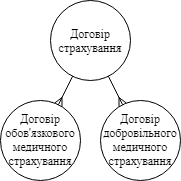
\includegraphics{idef_classification}
    \caption{Класифікація договорів страхування}
    \label{fig:idef_classification}
\end{figure}

\subsection*{Висновки}
У ході виконання лабораторної роботи було виконано аналіз предметної області, що пов'язана із управлінням страховими договорами. Була розроблена онтологія предметної області у вигляді діаграми взаємозв'язку, що відображає зв'язки між сутностями предметної області та діаграми станів. Також була розроблена фізична модель даних системи управління страховими договорами.

\end{document}
